% https://liam0205.me/2014/09/08/latex-introduction/index.html
% \开头的称为控制序列, 影响输出文档的效果, {}内为参数.
% 部分控制序列还有被[]包括的可选参数.
\documentclass[a4paper, 12pt]{article}
% \documentclass和\begin之间为`导言区`, 其中的控制序列一般影响整个输出文档.

% \usepackage{}用来调用宏包.

% 作者, 标题, 日期
% 使用`titling`可修改默认title格式
% http://texdoc.net/texmf-dist/doc/latex/titling/titling.pdf
\usepackage{titling}
\title{}
\author{Jin Dong}
% amsmath宏包提供数学功能.
% 公式分为inline($...$)和display(\[...\])两种模式.
% 若需要对公式编号, 使用equation模式\begin{equation}
\usepackage{amsmath}

% graphicx宏包的\includegraphics命令用于插入图片
\usepackage{graphicx}

\usepackage{subcaption}

\usepackage{float}

% 使用geometry宏包设置页边距
\usepackage{geometry}
% \geometry{papersize={20cm, 15cm}}
\geometry{left=2cm, right=2cm, top=2cm, bottom=2cm}

% 使用fancyhdr宏包设置页眉页脚
% http://texdoc.net/texmf-dist/doc/latex/fancyhdr/fancyhdr.pdf
\usepackage{fancyhdr}
\pagestyle{fancy}
\lhead{}
\chead{}
\rhead{}
%\lfoot{}
%\cfoot{\thepage}
%\rfoot{}
% 页眉和正文间的横线分割
\renewcommand{\headrulewidth}{0.4pt}
\renewcommand{\headwidth}{\textwidth}
\renewcommand{\footrulewidth}{0.4pt}

% 首行缩进两个中文汉字长度
%\usepackage{indentfirst}
%\setlength{\parindent}{\ccwd}

% 行间距通过setspace宏包调整, 如字号的1.5倍
\usepackage{setspace}
\onehalfspacing

% 段间距, 通过修改长度\parskip的值来调整
\addtolength{\parskip}{.4em}

\newcommand{\newAssignment}[2]{
	\begin{center}
  		\textbf{{\huge #1}}\vspace{10pt} \\
  		{\large #2}\vspace{15pt}
	\end{center}
}
% \newcommand{\newQuestion}[1]{\vspace{5pt}\textbf{\Large #1}}
\newcommand{\newQuestion}[1]{\section{#1}}
\newcommand{\newPart}[1]{\textbf{\large #1}}
\newcommand{\newImage}[2]{\includegraphics[width = #1\textwidth]{#2}}

\begin{document}

\newAssignment{COMP 512: Project 3 }{Group 14: Jin Dong, 260860634; Shiquan Zhang, 260850447}

\newQuestion{General design and architecture:} 

The distributed booking system mainly has three parts: Client, Middleware and three Remote Managers. The architecture of the system is shown in Figure 1.

\begin{figure}[H]
    \centering
    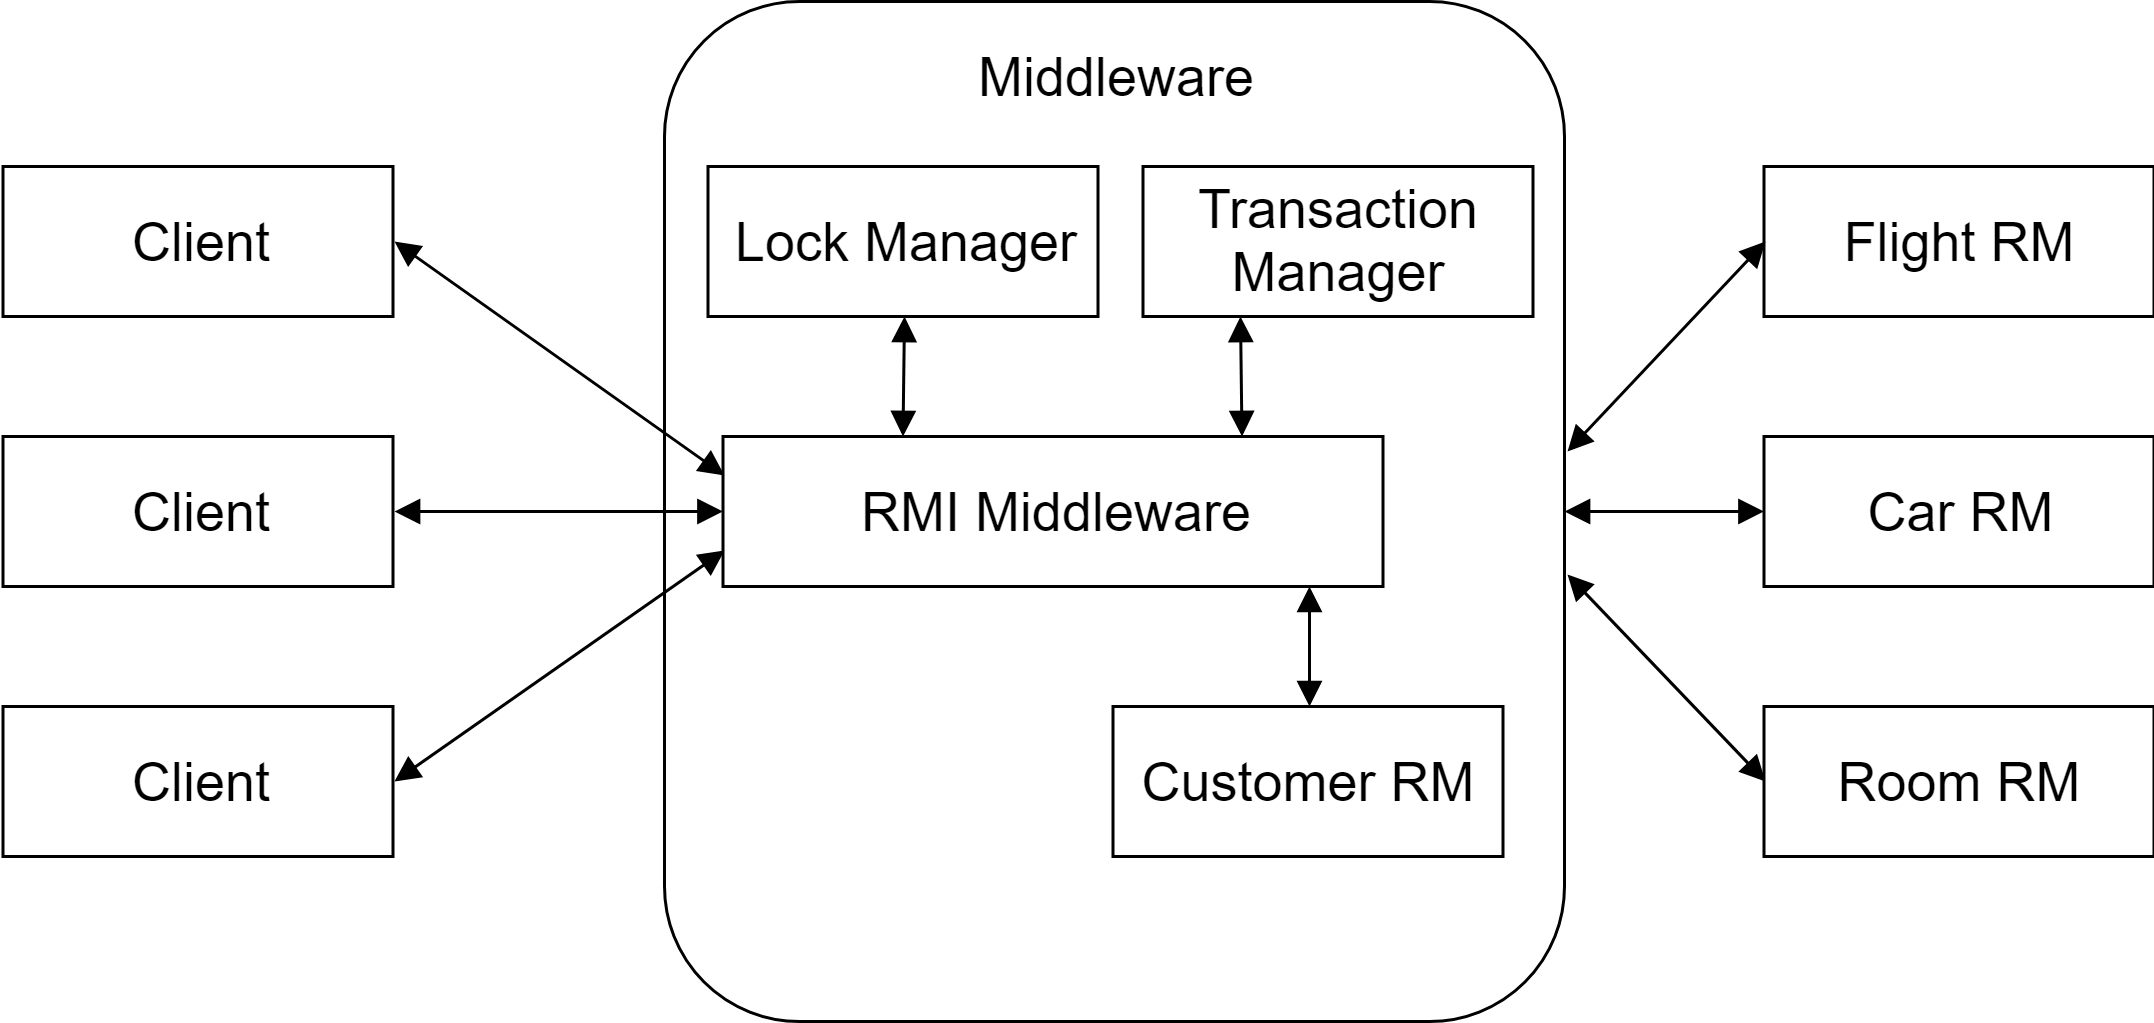
\includegraphics[width=0.8\linewidth]{Distributed_Booking_System.png}
    \caption{High-level Architecture of the System}
    \label{fig:Figure_1}
\end{figure}

\newPart{Client}

Client is directly communicate with clients. It deploys on the clients' machine and provides some APIs for clients, including 'AddCustomer', 'ReserveFlight', etc. It recieves commands from clients and proceeds them to the server (Middleware). 
After server finishing to process the commands, it recieves the execution results and prints out on the screen.

\newPart{Middleware}

Middleware is mainly consisted by four parts: RMIMiddleware, Transaction Manager, Lock Manager and Customer Remote Manager. 

1. RMIMiddleware is the only part of the server which directly communicates with Client. It exposes all APIs that Client needs and coordinates all of these commands in the server side. 

2. Transaction Manager mainly takes charge in the concurrency control of all transactions. It holds the transaction ID list and the corresponding RMs for every transaction. It also acts like the coordinator in the 2 Phase Commit.

3. Lock Manager ensures the data integrity among concurrent transactions. The system uses 2 Phase Locking algorithm and all locks of data are managed in the Lock Manager.

4. Customer RM takes charge in managing the data of the customers, including customer ID and reservations of every customer.

\newPart{Remote Managers (RM)}

There are three distributed databases deployed in three different remote machines, which are managed by three Resource Managers separately. They are Flight RM, Car RM and Room RM, which take charge in reading, writing and committing/aborting the data of flights, cars and rooms.

\newQuestion{Individual features:}

The distributed booking system has several features that insure it runs well when handling several transactions from different clients concurrently. Basically there are four main features: distribution and communication, transactions and locking (2PL), data shadowing and logging and recovery (2PC).

\newPart{Distribution and communication}

The booking system mainly has four types of data: customers, flights, cars and rooms, which are managed by four RMs. Three RMs are physically in three remote machine separately and the Customer RM is in the Middleware. When a normal operation of a transaction, i.e. \textit{add/delete/query/reserve}, comes in, Middleware records some information about this transaction, such as the corresponding RMs, in the Transaction manager. Then Middleware applies locks for this operation in the Lock manager. Next, it forwards the operation to the corresponding RMs. Finally, Middleware collects the results and returns them to the Client.

The system uses the Remote Method Invocation (RMI) in Java. The RM exposes several APIs that the Middleware can invocates them remotely and get the results from the resouce managers. So does that between Middleware and Client. The RMI method hides the details of network communication in the built-in RMI module and it's convenient to use.

\newPart{Transactions and locking (2PL)}

We implement a centralized lock manager, letting Middleware manage locks of all items. For each method a transaction calls, the Middleware will first call its \textit{lockSomething} method. The Transaction manager in the Middleware will first check if the transaction exists. If not, a \textit{InvalidTransactionException} will be thrown. Then the Lock manager will try to grant a corresponding lock on that item to the transaction. If either the lock granting failed or a DeadlockException is thrown, the Middleware will abort this transaction and throw a \textit{TransactionAbortedException}. Only the \textit{lockSomething} succeeds can the subsequent operations be executed. For example, in a \textit{reserveCar} operation, the middleware will try to grant a WRITE lock on the car and  a WRITE lock on the customer to this transaction. If both succeed, the real \textit{reserveCar} operation will be executed.

When a transaction request a lock on an item on which the transaction already has a lock, there are three situations that may happen: (1) request: READ, have: READ (2) request: WRITE, have: WRITE; (3) request: WRITE, have: READ. For (1) and (2), Lock Manager will raise\textit{RedundantLockRequestException} and return true. For (3), Lock Manager will first check if other transactions are granted locks on this item. If not, the Lock manager will delete the READ lock and grant a WRTIE lock to this transaction.

\newPart{Data shadowing}

In case that some parts of the system may crash sometime, the data must be preserve into the disk, as well as be written into a file. However, there are a lot of I/O operations in saving data. It might be problematic if the system crash during this period. To guarantee the safety of data, we use data shadowing in the system. 

When committing a transaction, both Middleware and RMs need to write some data to the disk. For every RM, there are two files shadowing the data, \textit{RMname.A} and \textit{RMname.B}. One is working file and the other is master records. There is a pointer indicating which file is the master records and which is the working file. Every time the RM executes commit transaction, it writes the transaction data to the working file. When finishing writing successfully, it flips the pointer from the original master records to the working file. And the original master records becomes the new working file. Besides, the pointer is preserved in another file, \textit{RMname.master}. If the system crash when writing data into the working file, the pointer doesn't change. Therefore, when the RM restarts, it recovers the data from the original master records and loads them into the memory.

\newPart{Logging and recovery (2-PC)}

To guarantee the data consistency during committing, we implement the two phase commit procedure, which includes some logging and recovery procedures. For the 2PC procedure, the log is writen in a independent file, \textit{name.log}.

When Client decides to commit a transaction, \textit{twoPC()} in the Middleware will be called. In the Middleware, the Transaction manager is the coordinator of 2-PC. First, it logs the \textit{"start-2PC"} information and calls the \textit{prepare()} in every RM corresponding to this transaction concurrently by starting multiple new threads. Then it logs the voting results in a Hashmap \textit{vote}. When the size of \textit{vote} equals to the number of corresponding RMs, voting finishes and the it checks the voting results. If all RM vote YES, it logs \textit{"COMMIT"} and calls the \textit{commit()} in every corresponding RM. Otherwise, it logs \textit{"ABORT"} and calls the \textit{abort()} in every RM voting YES.

If the Middleware crashes and restarts, it will execute \textit{restart()} automatically. In the recovery phase, the Middleware not only recovers the data from shadowing files, but also checks the 2PC log file. For every transaction logged in the file, the Middleware checks its status in 2PC. For the transactions with log \textit{"START-2PC"} and \textit{"ABORT"}, Middleware executes \textit{"abort()"}. For the transactions with log \textit{"COMMIT"}, Middleware executes \textit{commit()} again.

In the RM side, when the \textit{prepare()} is called, RM will check whether this transaction has been aborted in its records. If the transaction has been aborted, RM returns NO. Otherwise, it logs \textit{"YES"} and returns YES to the Middleware. When RM recieves the decision from the Middleware, as well as the \textit{commit()} or \textit{abort()} is called, RM will log \textit{"COMMIT"} or \textit{"ABORT"} and execute correspondingly.

If RM crashes and restarts, it will also execute \textit{restart()} automatically. Besides recovering data from the shadowing file, RM also reads the information from the 2PC log file. For every transaction in the log file, if it has the log \textit{"INIT"}, RM will aborts it. Otherwise, RM does nothing.

\newQuestion{Special features:} 

Besides the main features above, we also implement some special auxiliary features to strengthen the robustness of the system.

\newPart{Map from xid to related RMs in TransactionManager}

When Middleware reconnects to RMs after whoever crashes, we need to update the whole map if we store RM as a reference here. Instead, we only store the RM's name and add a small Hashtable which maps the name to the reference. So when reconnection happens, TransactionManager only need to update each reference one time at most.

\newPart{Crash detection}

Middleware need to detect the crash of RMs so that it can reconnect to the RM on time. We create a new Thread in which Middleware will ping the three RMs (send an empty message). Whenever this thread catches a RemoteException it knows that this RM crashed, so it will try to reconnect the RM and update the reference in TM.

\newPart{Time-to-Live mechanisim}

We implement this function by creating a new Thread in Middleware, which for-loop all active transactions and checks if System.currentTimeMillis() - xid\_time.get(xid) $>$ MAX\_EXIST\_TIME. If so, Middleware will abort this transaction. Client will know this abortion when it calls next operation on this transaction and catch a UnvalidTransactionException. We update xid\_time.get(xid) in the middleware's \textit{lockSomething} function because each operation will call Lock first.

\newQuestion{Problems:}

For the crash mode 3 in RM, it requires that RM should crash after sending the vote to the coordinator while before recieving the decision. In our implementation, we use RMI as the communication method between Middleware and RM, thus after returning the vote to the Middleware, the thread for \textit{prepare()} ends and there is no place to execute the crash operation. To solve this problem, we create a new thread at the end of the \textit{prepare()}. If the flag for creash mode 3 is up, this thread sleeps for 10 milliseconds to ensure the vote returns to the Middleware and then it executes \textit{System.exit(1)} to crash the RM.

\newQuestion{Testing:}

Testing mainly includes concurrency control test and crash/recover test.

\newPart{Concurrency control}

To test the locking mechanism, we test serveral examples in different aspects, including testing simple commit, simple abort, Customer lock, lock conversion, deadlock, time-to-live check, bundle atomicity and multiple operations using local copy. Take the deadlock test as an example, we starts two Clients simultaneously. One queries on item \textit{A} and adds on item \textit{B}, while the other queries on item \textit{B} and adds on item \textit{A}. Then both Clients are caught into a deadlock. After waiting for timeout, the first transaction will be aborted and the other will succeeds.

\newPart{Crash and recovery}

We insert breakpoints for 8 crash modes in the Middleware and for 5 crash modes in RM, which covers all critical operations in the 2PC procedure. When some of the flags for these breakpoints are true, the Middleware or RM will crash when committing a transaction. For different crash modes, the log information or the status of other servers might be different when one machine crashes. So we can test the data shadowing and recovery mechanism in 2PC procedure by crashing in different modes and restarting manually. After restarts the Middleware or RM that crashed, the Middleware/RM should be able to load the data back to memory from the shadowing file. And the decision for every transaction should also be consistent in Middleware and all RMs (committed or aborted).

% \maketitle
% \tableofcontents
% 在文章类article/ctexart中定义了五个控制序列来调整行文组织:
% section\{\}
% subsection\{\}
% subsubsection\{\}
% paragraph\{\}
% subparagraph\{\}
\end{document}